\documentclass[dvipdfmx]{jsarticle}
\usepackage{tikz}
\usetikzlibrary{calc, quotes, angles}%quotesは角度のラベルオプション内に記述するために使用
\begin{document}

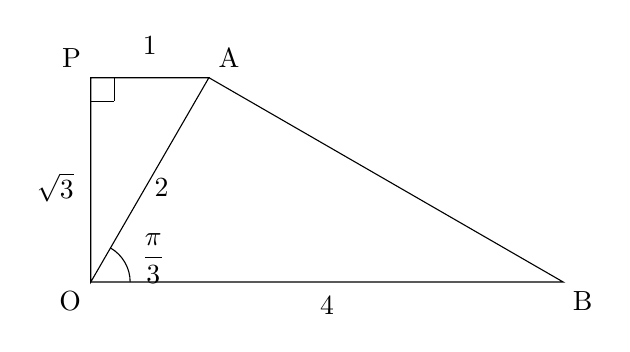
\begin{tikzpicture}[scale = 1.5]
 \draw
 (1,1.73) coordinate (A) node[above right] {A}
 -- (0,0) coordinate (O) node[below left] {O}
 -- (0, 1.73) coordinate (P) node[above left] {P}
 -- cycle;
 \coordinate (Q) at ($(P)!.2cm!(O)!.2cm!90:(O)$);%直角記号の頂点の設定
 \draw[thin] ($(A)!(Q)!(P)$)--(Q);
 \draw[thin] ($(P)!(Q)!(O)$)--(Q);
 \draw
 (A)
 -- (4,0) coordinate (B) node[below right] {B}
 -- (O) 
 pic["$\displaystyle \frac{\pi}{3}$", draw, -, thin, angle eccentricity=1.2, angle radius=0.5cm, right] {angle=B--O--A};
 \node(AP) at (0.5,2) {$1$};
 \node(OP) at ( -0.3,0.8) {$\sqrt{3} $};
 \node(OA) at ( 0.6,0.8) {$2$};
 \node(OB) at ( 2, - 0.2) {$4$};
\end{tikzpicture}

\begin{tikzpicture}[scale = 1.5]
 \draw
 (1.773, -1) coordinate (A) node[right] {A}
 -- (0,0) coordinate (O) node[left] {O}
 -- ( 1.73/2, - 1.5) coordinate (P) node[below left] {P}
 -- cycle;
 \coordinate (Q) at ($(P)!.2cm!(O)!.2cm!90:(P)$);%直角記号の頂点の設定
 \draw ($(A)!(Q)!(P)$)--(Q);
 \draw ($(P)!(Q)!(O)$)--(Q);
 \draw
 (A)
 -- (1.73*2,2) coordinate (B) node[right] {B}
 -- (O) 
 pic["$\displaystyle \frac{\pi}{3}$", draw, -, thin, angle eccentricity=1.2, angle radius=0.5cm, right] {angle=A--O--B};
 \node(AP) at (1.5, - 1.5) {$1$};
 \node(OP) at ( 0.1, - 1) {$\sqrt{3} $};
 \node(OA) at ( 1.1, -0.3) {$2$};
 \node(OB) at ( 1.5, 1.1) {$4$};
\end{tikzpicture}


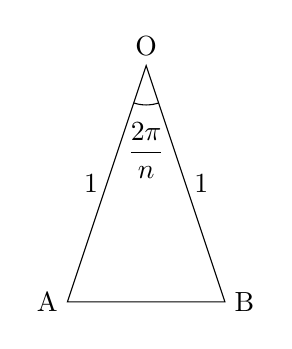
\begin{tikzpicture}[scale = 1]
 \draw
 (0, -3) coordinate (A) node[left] {A}
 -- (1,0) coordinate (O) node[above] {O}

 -- (2, -3) coordinate (B) node[right] {B}
 pic["$\displaystyle \frac{2\pi}{n}$", draw, -, thin, angle eccentricity=1.2, angle radius=0.5cm, below] {angle=A--O--B}
 -- cycle;
\node(OA) at (0.3, -1.5) {$1$};
\node(OB) at ( 1.7, - 1.5) {$1$};
\end{tikzpicture}


\end{document}

















